% -*- coding: utf-8 -*-
%%%%%%%%
% To control hyperref on command line,
% you can select one of (1),(2a),(2b),(3).
%   (1) do not treat hyperref
%   $ uplatex bkmk-utf8.tex
%   (2a) hyperref + dvipdfmx (with CMap conversion)
%   $ uplatex "\def\withhyperref{dvipdfmx}\input" bkmk-utf8.tex
%   (2b) hyperref + dvipdfmx + "convbkmk.rb -o"/out2uni (w/o CMap conversion)
%   $ uplatex "\def\withhyperref{dvipdfmx}\def\nocmap{true}\input" bkmk-utf8.tex
%   (3) hyperref + dvips + convbkmk.rb + distiller/ps2pdf
%   $ uplatex "\def\withhyperref{dvips}\input" bkmk-utf8.tex
%%%%%%

\newif\ifuptexmode\uptexmodefalse
\ifnum\jis"2121="3000

 %% for upLaTeX
 \def\pLaTeXorupLaTeX{upLaTeX}
 \uptexmodetrue
 \def\innerencoding{UPTEX}
 \def\cmap{UTF8-UTF16}

\else

 %% for pLaTeX
 \def\pLaTeXorupLaTeX{pLaTeX}
 \uptexmodefalse

 \ifnum\jis"2121="A1A1
  \def\innerencoding{EUC}
  \def\cmap{EUC-UCS2}
 \fi
 \ifnum\jis"2121="8140
  \def\innerencoding{SJIS}
  \def\cmap{90ms-RKSJ-UCS2}
 \fi

\fi

\makeatletter

\def\@opt@{multi}
\def\@default{default}
\def\@jarticle{jarticle}
\def\@tarticle{tarticle}
\def\@ujarticle{ujarticle}

\ifx\option\@undefined
 \def\option{default}
\fi

\ifx\class\@undefined
 \ifuptexmode
  \def\class{ujarticle}
 \else
  \def\class{jarticle}
 \fi
\fi
\ifuptexmode
 \edef\@opt@{uplatex,\@opt@}
\fi
\ifx\class\@jarticle
  \documentclass[a4paper,titlepage]{\class}
\else
 \ifx\class\@ujarticle
  \documentclass[a4paper,titlepage]{\class}
 \else
  \documentclass[a4paper,titlepage,landscape]{\class}
 \fi
\fi

\usepackage{graphicx}
\usepackage{textcomp}
\usepackage[\@opt@]{otf}

\def\@dvipdfmx{dvipdfmx}
\def\@dvips{dvips}

\ifx\withhyperref\@undefined
 \def\withhyperref{undefined}
 \def\texorpdfstring{%
   \expandafter\@firstoftwo
 }
\else
 \ifx\withhyperref\@dvipdfmx
  \def\@hyperrefkeyval{dvipdfm}
  \usepackage{atbegshi}
  \ifx\nocmap\@undefined
   \AtBeginShipoutFirst{\special{pdf:tounicode \cmap}}
  \else
   \def\cmap{---}
  \fi
 \fi
 \ifx\withhyperref\@dvips
  \def\@hyperrefkeyval{dvips}
 \fi

\ifx\nocmap\@undefined
 \usepackage[\@hyperrefkeyval,%
 bookmarks=true,%
 bookmarksnumbered=true,%
 bookmarkstype=toc,%
 %pdfstartview={FitBH -32768},%
 pdftitle={いろいろ確かめてみる},%
 pdfsubject={hyperref編},%
 pdfauthor={名無 権兵衛},%
 pdfkeywords={TeX; dvips; dvipdfmx; bookmark; hyperref; しおり; pdf}%
 ]{hyperref}
\else
 \input bkmk-docinfo.out
 \usepackage[dvipdfm,%
 bookmarks=true,%
 bookmarksnumbered=true,%
 bookmarkstype=toc,%
 %pdfstartview={FitBH -32768},%
 pdftitle=\PDFTITLE,%
 pdfsubject=\PDFSUBJECT,%
 pdfauthor=\PDFAUTHOR,%
 pdfkeywords=\PDFKEYWORDS%
 ]{hyperref}
\fi

\fi

\makeatother


%%% for upLaTeX only
\ifuptexmode
\DeclareFontFamily{JY2}{mcw}{}
\DeclareFontFamily{JY2}{gtw}{}
\DeclareFontShape{JY2}{mcw}{m}{n}{<->s*[0.962216]upjpnrm-h}{}
\DeclareFontShape{JY2}{gtw}{m}{n}{<->s*[0.962216]upjpngt-h}{}
\DeclareFontShape{JY2}{gt}{m}{n}{<->s*[0.962216]upjpngt-h}{}
\DeclareFontShape{JY2}{mcw}{bx}{n}{<->ssub*gt/m/n}{}
\DeclareFontShape{JY2}{gtw}{bx}{n}{<->ssub*gt/m/n}{}
\DeclareFontShape{JY2}{gt}{bx}{n}{<->ssub*gt/m/n}{}
\DeclareRobustCommand\mcw{\kanjifamily{mcw}\selectfont}
\DeclareRobustCommand\gtw{\kanjifamily{gtw}\selectfont}
\renewcommand\mcdefault{mcw}
\renewcommand\gtdefault{gtw}

\DeclareFontFamily{JY2}{schrm}{}
\DeclareFontFamily{JY2}{tchrm}{}
\DeclareFontFamily{JY2}{korrm}{}
\DeclareFontShape{JY2}{schrm}{m}{n}{<->s*[0.962216]upschrm-h}{}
\DeclareFontShape{JY2}{tchrm}{m}{n}{<->s*[0.962216]uptchrm-h}{}
\DeclareFontShape{JY2}{korrm}{m}{n}{<->s*[0.962216]upkorrm-h}{}
\DeclareFontShape{JY2}{schrm}{bx}{n}{<->ssub*schrm/m/n}{}
\DeclareFontShape{JY2}{tchrm}{bx}{n}{<->ssub*tchrm/m/n}{}
\DeclareFontShape{JY2}{korrm}{bx}{n}{<->ssub*korrm/m/n}{}
\DeclareRobustCommand\schrm{\kanjifamily{schrm}\selectfont}
\DeclareRobustCommand\tchrm{\kanjifamily{tchrm}\selectfont}
\DeclareRobustCommand\korrm{\kanjifamily{korrm}\selectfont}
\fi

\title{いろいろ確かめてみる}

\author{名無 権兵衛}

\oddsidemargin0mm
\evensidemargin0mm
\topmargin-15mm
\textwidth162mm
\textheight245mm

\edef\bs{$\backslash$\kern0em}

\begin{document}
\maketitle
\section{section title by ASCII}
test test.

hyperref with: \withhyperref
\makeatletter
\ifx\withhyperref\@dvipdfmx
 ~~CMap:\cmap
\fi
\makeatother
\typeout{### hyperref with: \withhyperref}

pLaTeX or upLaTeX: \pLaTeXorupLaTeX
\typeout{### pLaTeX or upLaTeX: \pLaTeXorupLaTeX}

inner encoding: \innerencoding
\typeout{### inner encoding: \innerencoding}

\begin{figure}
 \begin{center}
  \scalebox{0.2}{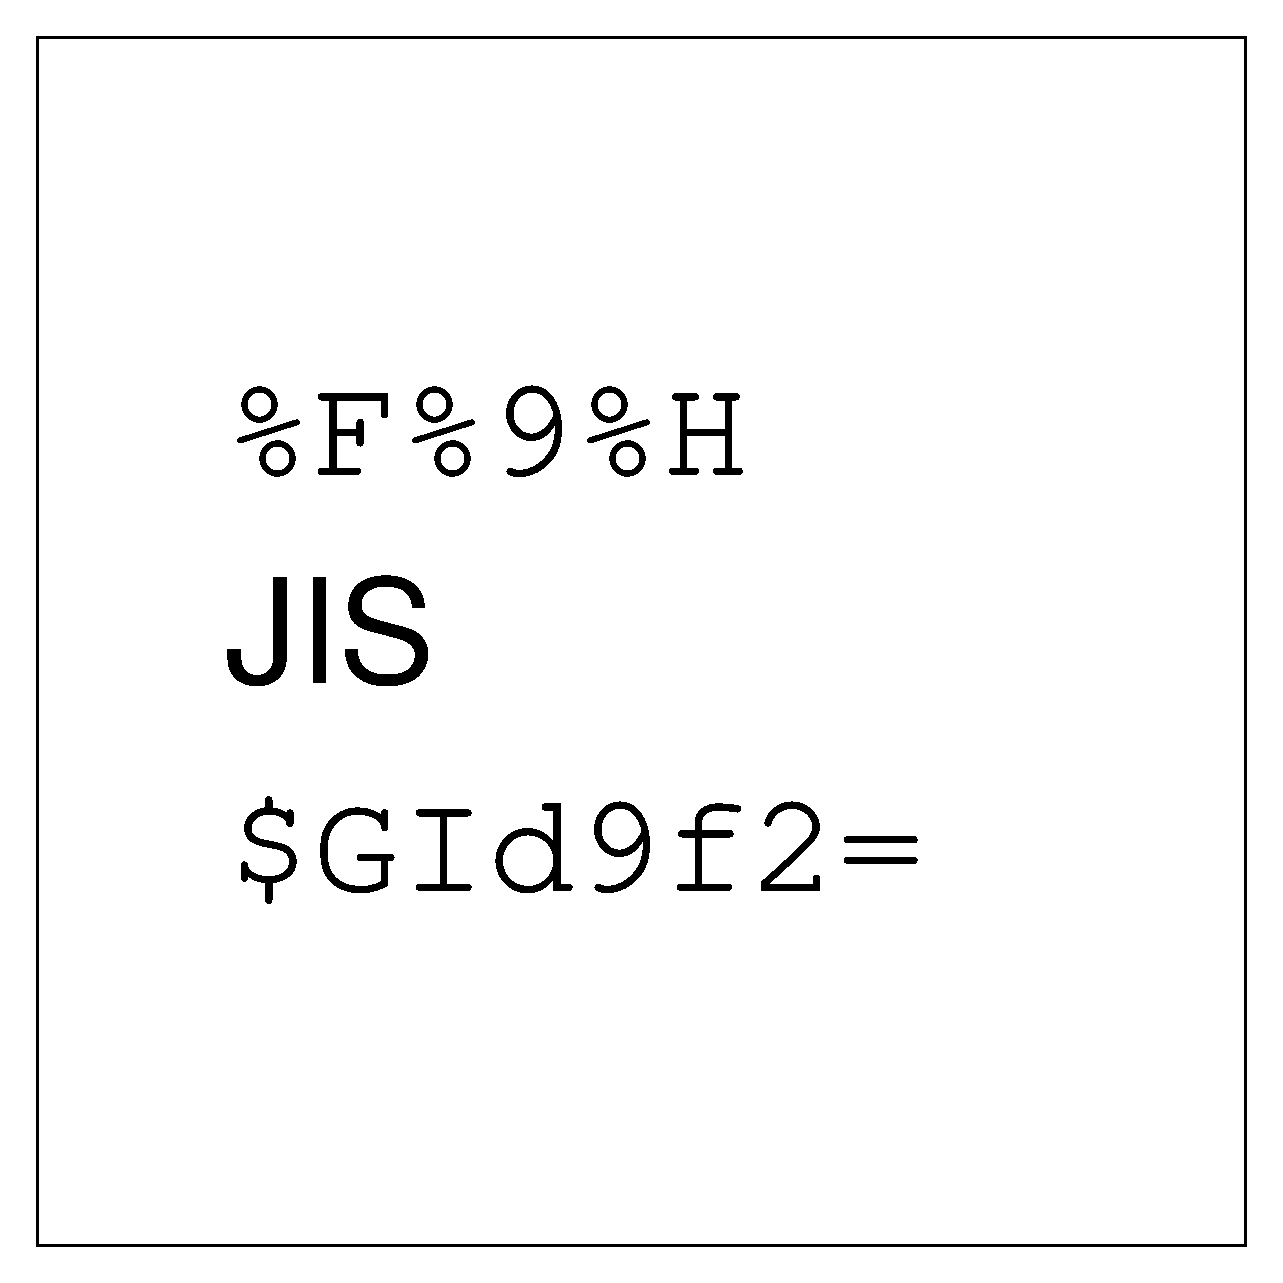
\includegraphics{box-jis.eps}}
  \caption{JISで符号化されたEPSファイル}
  \label{fig:box-jis}
 \end{center}
\end{figure}
%\begin{figure}
% \begin{center}
%  \scalebox{0.2}{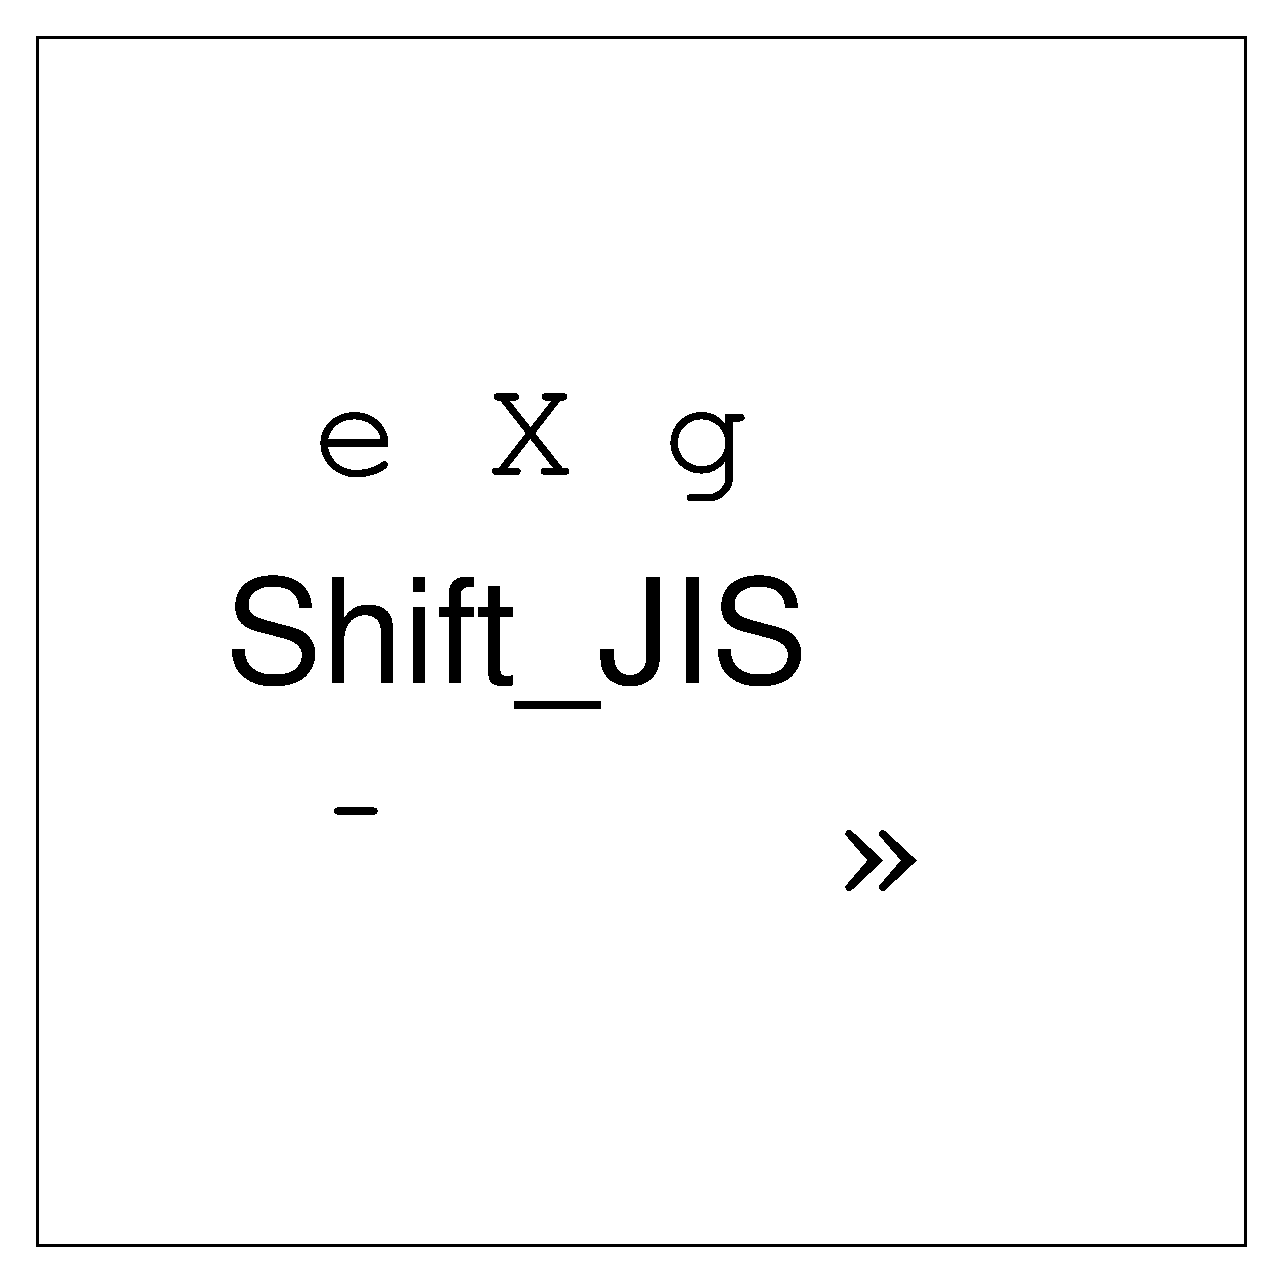
\includegraphics{box-sjis.eps}}
%  \caption{Shift\_JISで符号化されたEPSファイル}
%  \label{fig:box-sjis}
% \end{center}
%\end{figure}
%\begin{figure}
% \begin{center}
%  \scalebox{0.2}{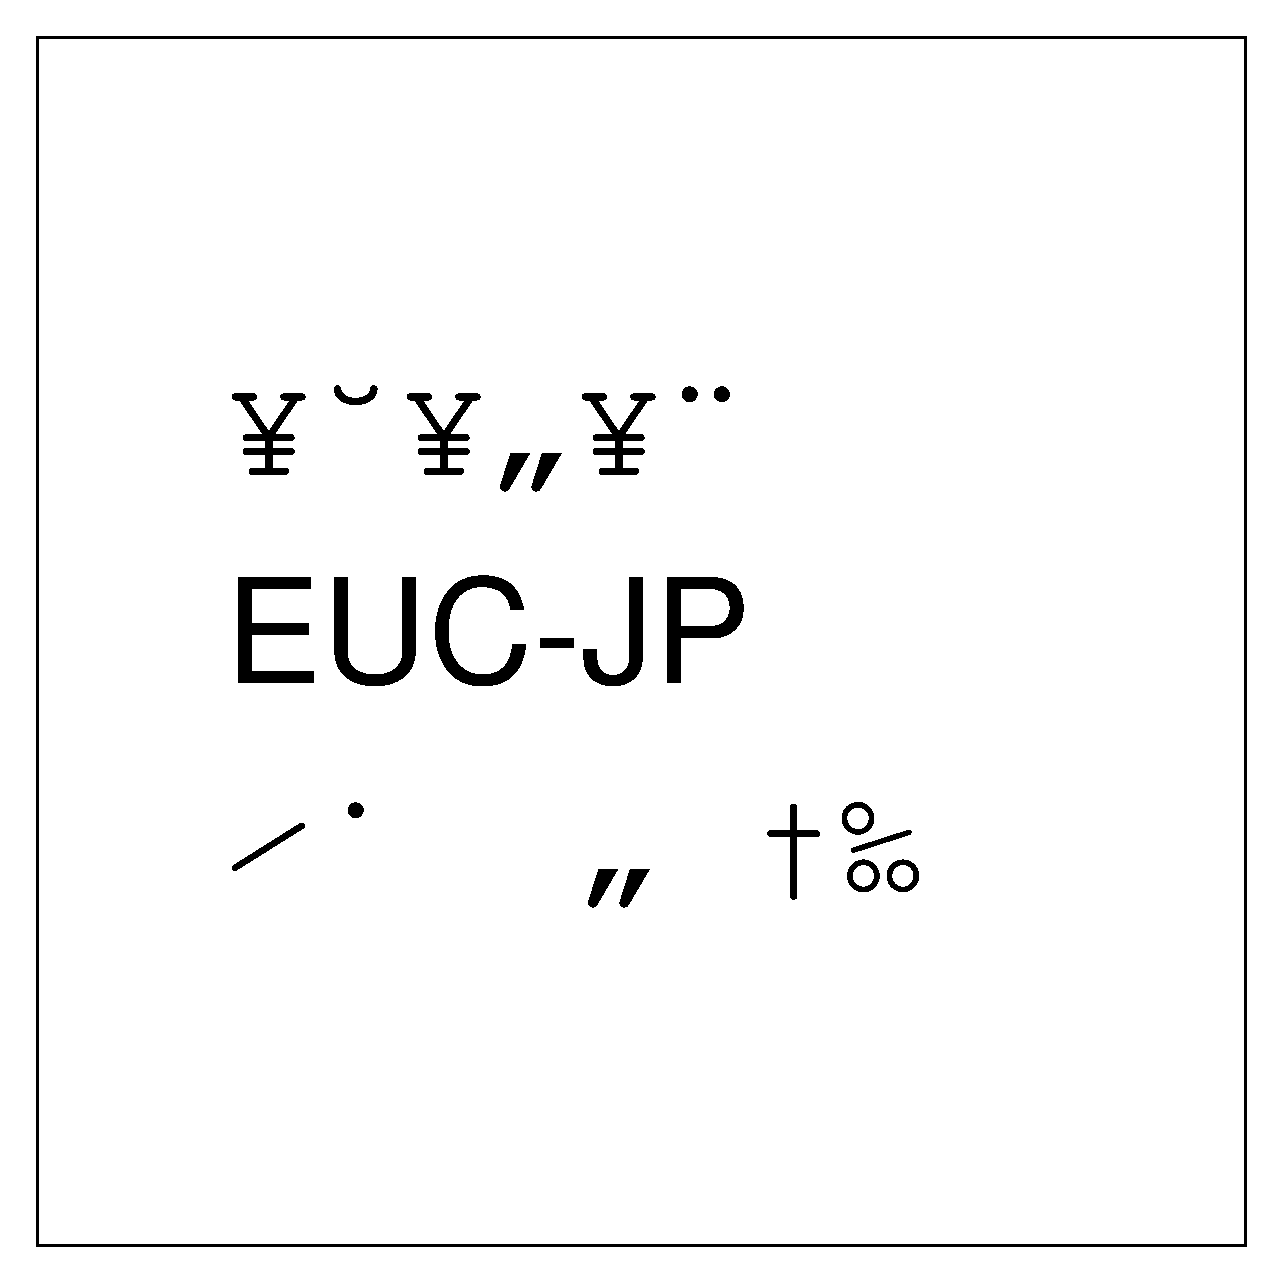
\includegraphics{box-euc.eps}}
%  \caption{EUC-JPで符号化されたEPSファイル}
%  \label{fig:box-euc}
% \end{center}
%\end{figure}
%\begin{figure}
% \begin{center}
%  \scalebox{0.2}{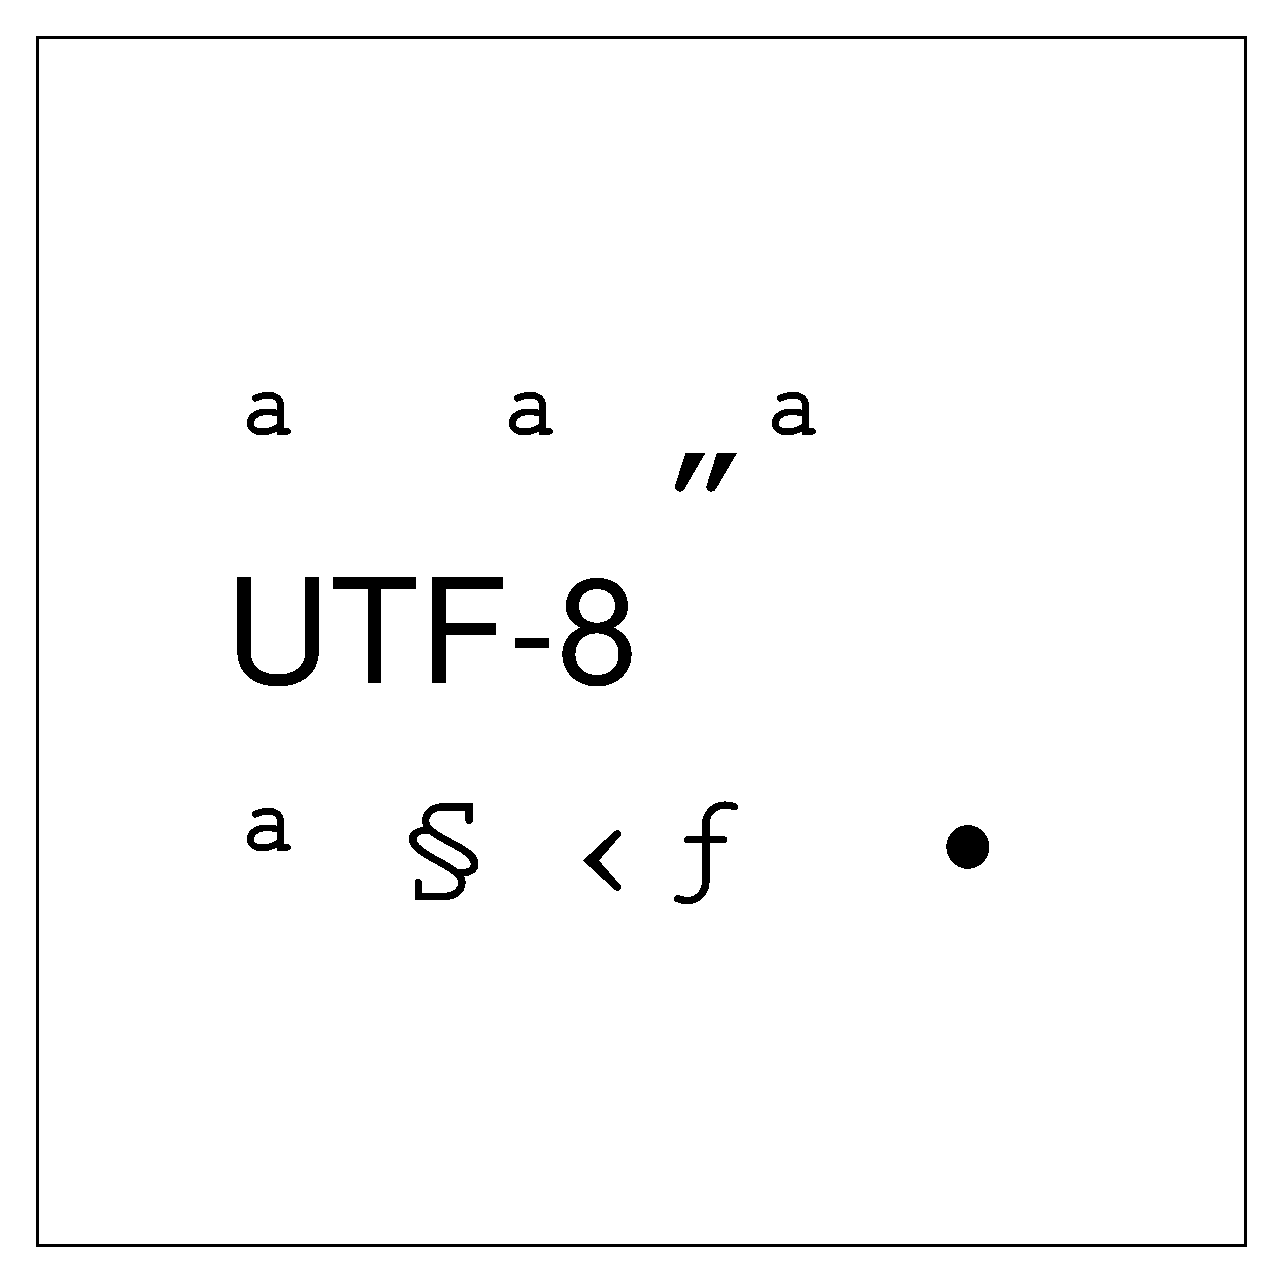
\includegraphics{box-utf8.eps}}
%  \caption{UTF-8で符号化されたEPSファイル}
%  \label{fig:box-utf8}
% \end{center}
%\end{figure}
\section{αβγ}
test test.

\section{абв}
test test.

\section{セクション}
test test.
\subsection{サブセクション(括弧)}
test test.

\makeatletter
\ifx\withhyperref\@undefined
\else

\section{Escape sequences \texorpdfstring{\textbullet\textdagger\textdaggerdbl\ldots---\textflorin--\textperthousand\texttrademark\texteuro}%
{\200\201\202\203\204\206\205\213\222\240}など}
\textbullet\textdagger\textdaggerdbl\ldots---\textflorin--\textperthousand\texttrademark\texteuro など

\section{見出しに\texorpdfstring{\bs}{\134}UTF, \texorpdfstring{\bs}{\134}UTFC, \texorpdfstring{\bs}{\134}UTFMなど}
\subsection{日本:\UTF{9aa8}\UTF{6D77} 簡体字:\UTFC{9aa8}\UTFC{6D77} 繁體字:\UTFT{9AA8}\UTFT{6d77} 朝鮮:\UTFK{9AA8}\UTFK{6d77}}
日本:\UTF{9aa8}\UTF{6D77} 簡体字:\UTFC{9aa8}\UTFC{6D77} 繁體字:\UTFT{9AA8}\UTFT{6d77} 朝鮮:\UTFK{9AA8}\UTFK{6d77}

\subsection{ハングル:\UTFK{c548}\UTFK{b155}\UTFK{d558}\UTFK{C138}\UTFK{C694}}
ハングル:\UTFK{c548}\UTFK{b155}\UTFK{d558}\UTFK{C138}\UTFK{C694}

\subsection{日本:\UTF{20509}\UTF{241FE} 簡体字:\UTFC{20509}\UTFC{241FE}  多言語:\UTFM{20509}\UTFM{241FE}}
日本:\UTF{20509}\UTF{241FE} 簡体字:\UTFC{20509}\UTFC{241FE}  多言語:\UTFM{20509}\UTFM{241FE}

\subsection{日本:\UTF{20509}\UTF{241FE} 簡体字:\UTFC{20509}\UTFC{241FE}  多言語:\UTFM{20509}\UTFM{241FE}}
日本:\UTF{20509}\UTF{241FE} 簡体字:\UTFC{20509}\UTFC{241FE}  多言語:\UTFM{20509}\UTFM{241FE}

\subsection{日本:\UTF{20b9f}\UTF{26402} 繁體字:\UTFT{20b9f}\UTFT{26402}  多言語:\UTFM{20b9f}\UTFM{26402}}
日本:\UTF{20b9f}\UTF{26402} 繁體字:\UTFT{20b9f}\UTFT{26402}  多言語:\UTFM{20b9f}\UTFM{26402}

\subsection{簡体字:\UTFC{20087}\UTFC{200cc} 繁體字:\UTFT{20087}\UTFT{200cc}  多言語:\UTFM{20087}\UTFM{200cc}}
簡体字:\UTFC{20087}\UTFC{200cc} 繁體字:\UTFT{20087}\UTFT{200cc}  多言語:\UTFM{20087}\UTFM{200cc}
\fi
\makeatother

%%% for upLaTeX only
\ifuptexmode
\section{以下は、upLaTeXのみ}
\subsection{いわゆる『新JIS』『JIS2004』: ♫♡☗〠☎☃♨①❷⓷ⅳⅤⓐ㋑}
便利な記号がいっぱい。

\subsection{Extension B (BMP外)の文字: 𠀋𠆢𠘨𡈽𠮟など}
𠂉𠀋𠂢𠂤𠆢𠈓𠌫𠎁𠍱𠏹𠑊𠔉𠗖𠘨𠝏𠠇𠠺𠢹𠥼𠦝
𠫓𠬝𠵅𠷡𠺕𠹭𠹤𠽟𡈁𡈽𡉕𡉻𡉴𡋤𡋗𡌛𡋽𡌶𡍄𡏄
𡑮𡑭𡗗𦰩𡙇𡜆𡝂𡢽𡧃𡱖𡴭𡚴𡵅𡵸𡵢𡶡𡶜𡶒𡶷𡷠
𡸴𡸳𡼞𡽶𡿺𢅻𢌞𢎭𢛳𢡛𢢫𢦏𢪸𢭏𢭐𢭆𢰝𢮦𢰤𢷡
𣇄𣇃𣇵𣆶𣍲𣏓𣏒𣏐𣏤𣏕𣏚𣏟𣑊𣑑𣑋𣑥𣓤𣕚𣗄𣖔
𣘹𣙇𣘸𣘺𣜿𣜜𣝣𣜌𣝤𣟿𣟧𣠤𣠽𣪘𣱿𣳾𣴀𣵀𣷺𣷹
𣷓𣽾𤂖𤄃𤇆𤇾𤎼𤘩𤚥𤟱𤢖𤩍𤭖𤭯𤰖𤴔𤸎𤸷𤹪𤺋
𥁊𥁕𥄢𥆩𥇥𥇍𥈞𥉌𥐮𥒎𥓙𥔎𥖧𥝱𥞩𥞴𥧄𥧔𥫤𥫣
𥫱𥮲𥱋𥱤𥶡𥸮𥹖𥹥𥹢𥻘𥻂𥻨𥼣𥽜𥿠𥿔𦀌𥿻𦀗𦁠
𦃭𦉰𦊆𦍌𣴎𦐂𦙾𦚰𦜝𦣝𦣪𦥑𦥯𦧝𦨞𦩘𦪌𦪷𦫿𦱳
𦳝𦹀𦹥𦾔𦿸𦿶𦿷𧃴𧄍𧄹𧏛𧏚𧏾𧐐𧑉𧘕𧘔𧘱𧚄𧚓
𧜎𧜣𧝒𧦅𧪄𧮳𧮾𧯇𧲸𧶠𧸐𧾷𨂊𨂻𨉷𨊂𨋳𨏍𨐌𨑕
𨕫𨗈𨗉𨛗𨛺𨥉𨥆𨥫𨦇𨦈𨦺𨦻𨨞𨨩𨩱𨩃𨪙𨫍𨫤𨫝
𨯁𨯯𨴐𨵱𨷻𨸟𨸶𨺉𨻫𨼲𨿸𩊠𩊱𩒐𩗏𩙿𩛰𩜙𩝐𩣆
𩩲𩷛𩸽𩸕𩺊𩹉𩻄𩻩𩻛𩿎𪀯𪀚𪃹𪂂𪆐𢈘𪎌𪐷𪗱𪘂
𪘚𪚲𠮟\\

\subsection[中国語・簡体字 简体中文]{中国語・簡体字 {\schrm 简体中文}}
{\schrm 简体中文}

\subsection[中国語・繁体字 繁體中文]{中国語・繁体字 {\tchrm 繁體中文}}
{\tchrm 繁體中文}

\subsection[韓国語  한국어]{韓国語 {\korrm 한국어}}
{\korrm 한국어}

\subsection{半角カタカナ}
半角カタカナ
\fi

\end{document}
